\section{Image processing}

Support for visual processing is a mandatory requirement for a
software library designed to be used in humanoid robotics. Real time
systems are critical for vision, as computer vision algorithms require
the elaboration of a large quantity of data.

Efficiency is very important in image processing, so we choose
an approach which interfaces particularly well with popular
optimized libraries, but which is still capable of good
performance in their absence.

To help developers write efficient visual processing routines, Intel
released the Image Processing Library (IPL). This library in optimized
to provide high performance on machines which employ Intel processors,
especially if equipped with MMX\texttrademark technology. The IPL
library is a set of C functions which implement basic operations on
images, from simple algebraic operations on pixels to color
conversions and convolutions. The library consists of different
modules optimized for different CPU. For better performance at
run-time the library automatically detects the CPU type and loads the
module that is more suitable. Another advantage of using the IPL is
that it is at the core of the OpenCV library
(http://sourceforge.net/projects/opencvlibrary/) which provides 
sophisticated routines for image processing such as filtering, face
tracking, optic flow, and much more.

Our basic image class (YARPImage) has an internal structure that is
compatible with the IPL library.  This allows any user to take full
advantage of the IPL and/or OpenCV libraries; if these libraries
are not used, then a core set of functions are available through
YARP.  Furthermore, the image class can act as a {\em proxy} to image
data stored in a foreign format.  This is useful to prevent unnecessary
copies when using other image processing libraries, or interfacing
with image sources (e.g. framegrabbers) and sinks (e.g. a graphic
display).


%% Unfortunately the IPL library does not provide support for object
%% oriented programming. We decided to write a library which implements a
%% set of classes to store and manipulate the pixels of an image. The set
%% of classes is in the form of a C++ template that can be instantiated
%% for each pixel type (for example at the moment RGB, grayscale and
%% floating point are implemented). The YARPImageOf template defines an
%% interface for all the image classes in the library; as in other parts
%% of the library we decided to use templates for efficiency reasons. The
%% internal structure of the image is identical to the one used by the
%% IPL library. 


YARP also provides support for transmitting images between two YARP
ports.


\begin{figure}[t]
\centerline{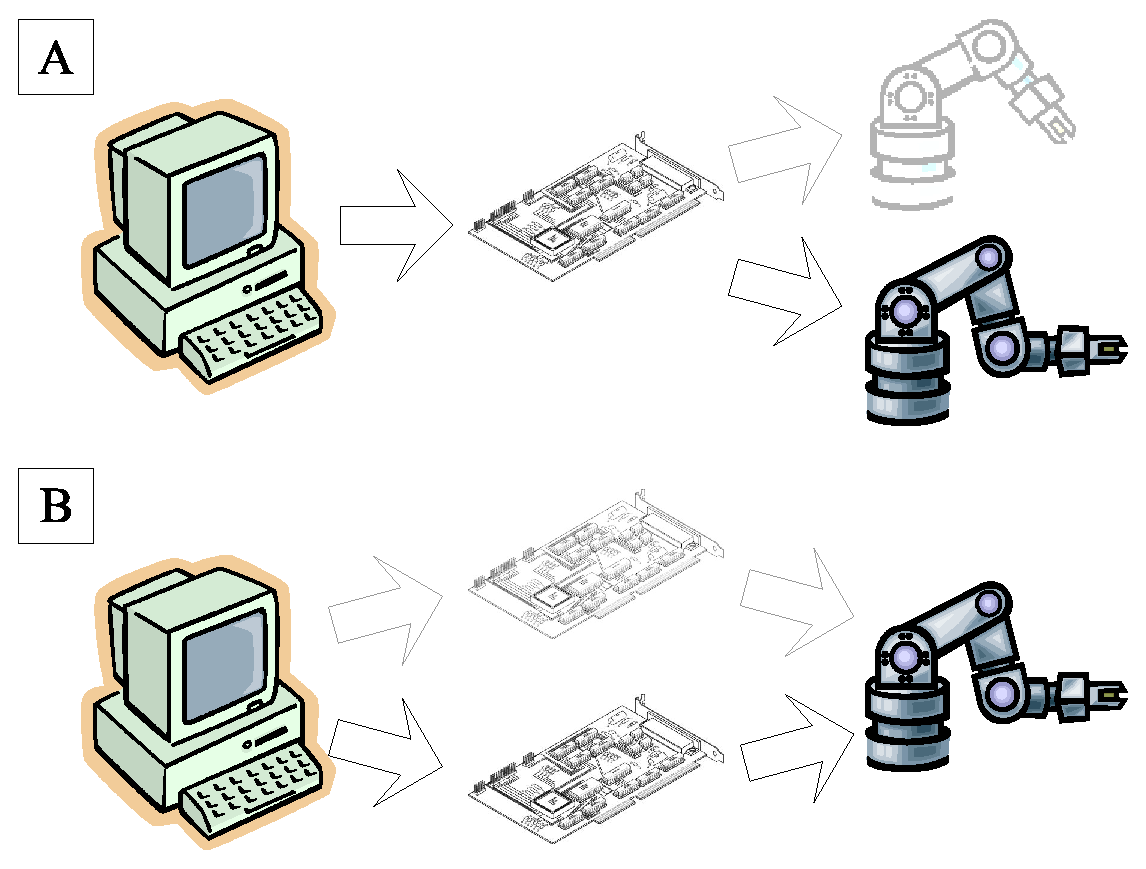
\includegraphics[width=\columnwidth]{fig-devices}}
\caption{
Changes in hardware make code reuse challenging.
YARP makes a distinction between {\em proximate} devices,
such as control boards and framegrabbers which are used to
talk to {\em distal} devices such as arms or sensors.  The 
same proximate device may be used to interface with different
distal devices (A).   Conversely, a given distal device may be
interfaced with using a choice of proximate devices (B).
Taking care to disentangle these two devices aids code reuse.
}
\label{fig:devices}
\end{figure}

\section{Device drivers}

A frequent problem encountered during development in robotics is that
it is very hard to reuse code on different platforms. In some
cases this cannot be avoided, especially when the platforms are
mechanically different. In other cases, however the platforms are
mechanically similar, and just have differences in their 
electronics~-- different frame grabbers, different
control boards, etc (see Figure~\ref{fig:devices}). 
In these situations it is not possible to reuse code
written for a platform on the other unchanged. 
However something can be done to
reduce the differences and localize them to specific components
by minimizing the degree to which
high level software modules are 
concerned with the low level details of the underlying hardware
platform.

The low level software should capture the essential functioning of the
particular class of device and hide the details of the
implementation. For example the device driver for a control board
should provide methods for moving a joint by specifying the desired
position, velocity and acceleration. Other common functionalities are
methods to read position, speed and torque (if available). In practice
the main differences between cards lay on the steps required for the
initialization of the device. This approach has been successful with
general purpose hardware like frame grabbers and control boards but
might fail to scale to custom devices like dedicated DSP for motion
control. In these cases it is harder (if not impossible) to identify a
common interface and it is best to provide a separate set of functions
to handle the specific functionalities of each device.

Another problem occurs when two identical boards are used
on setups that are mechanically different. Experience shows that in
these situations code reuse is very difficult. Consider for instance
the example of two robotic arms controlled by identical boards. The
calibration of the joints might be different if indexes are available
in the encoders or if hardware limits are presents in the
joints. Likewise, the procedure required to activate the amplifiers
might differ in the two cases. These dissimilarities cannot be handled
by different configuration files as they imply the execution of
different routines.

The ensemble of these routines are grouped in the adapter. This class
is in general responsible of implementing methods to correctly
initialize and quit the device, but it can implement other
functionalities as well. The adapter is hence the place where all the
peculiarities of each piece of hardware (and of the device used to
interface to it) are handled. As such it collects all and the only
routines specific to each hardware device.

Finally, device driver and adapter are aggregated together by a single
class. The interface between higher level software modules and the
hardware occurs through this class and is thus independent of the
device driver or the actual hardware underneath. Code changes required
to use different boards or mechanical devices are localized to the
device driver and the adapter respectively.

We defined a virtual device driver interface into YARP and
encapsulated the control parts of the robot into a standardized
template class hierarchy. The structure of the YARP virtual device
driver resembles the structure of UNIX device drivers. It has three
main methods: Open, Close and Ioctl. Open and Close execute code to
initialize and quit the device, whereas the IOCtl is the core of the
interface and consists in a set of messages. Each message defines an
index in a table of functions. The advantage of using this structure
as opposed to a virtual class is that it is not mandatory to implement
all methods if some are not supported by the hardware.

